\documentclass[border=0pt]{standalone}
\usepackage{verbatim}

\usepackage{pgfpages}
\usepackage{tikz}
\usetikzlibrary{arrows}
\usepackage{color}
\usepackage[utf8]{inputenc}

\tikzset{
	pindot/.style = {circle, draw=red, thick, minimum width=0.2, inner sep = 2pt},
}

\begin{document}
	\bf \tt
	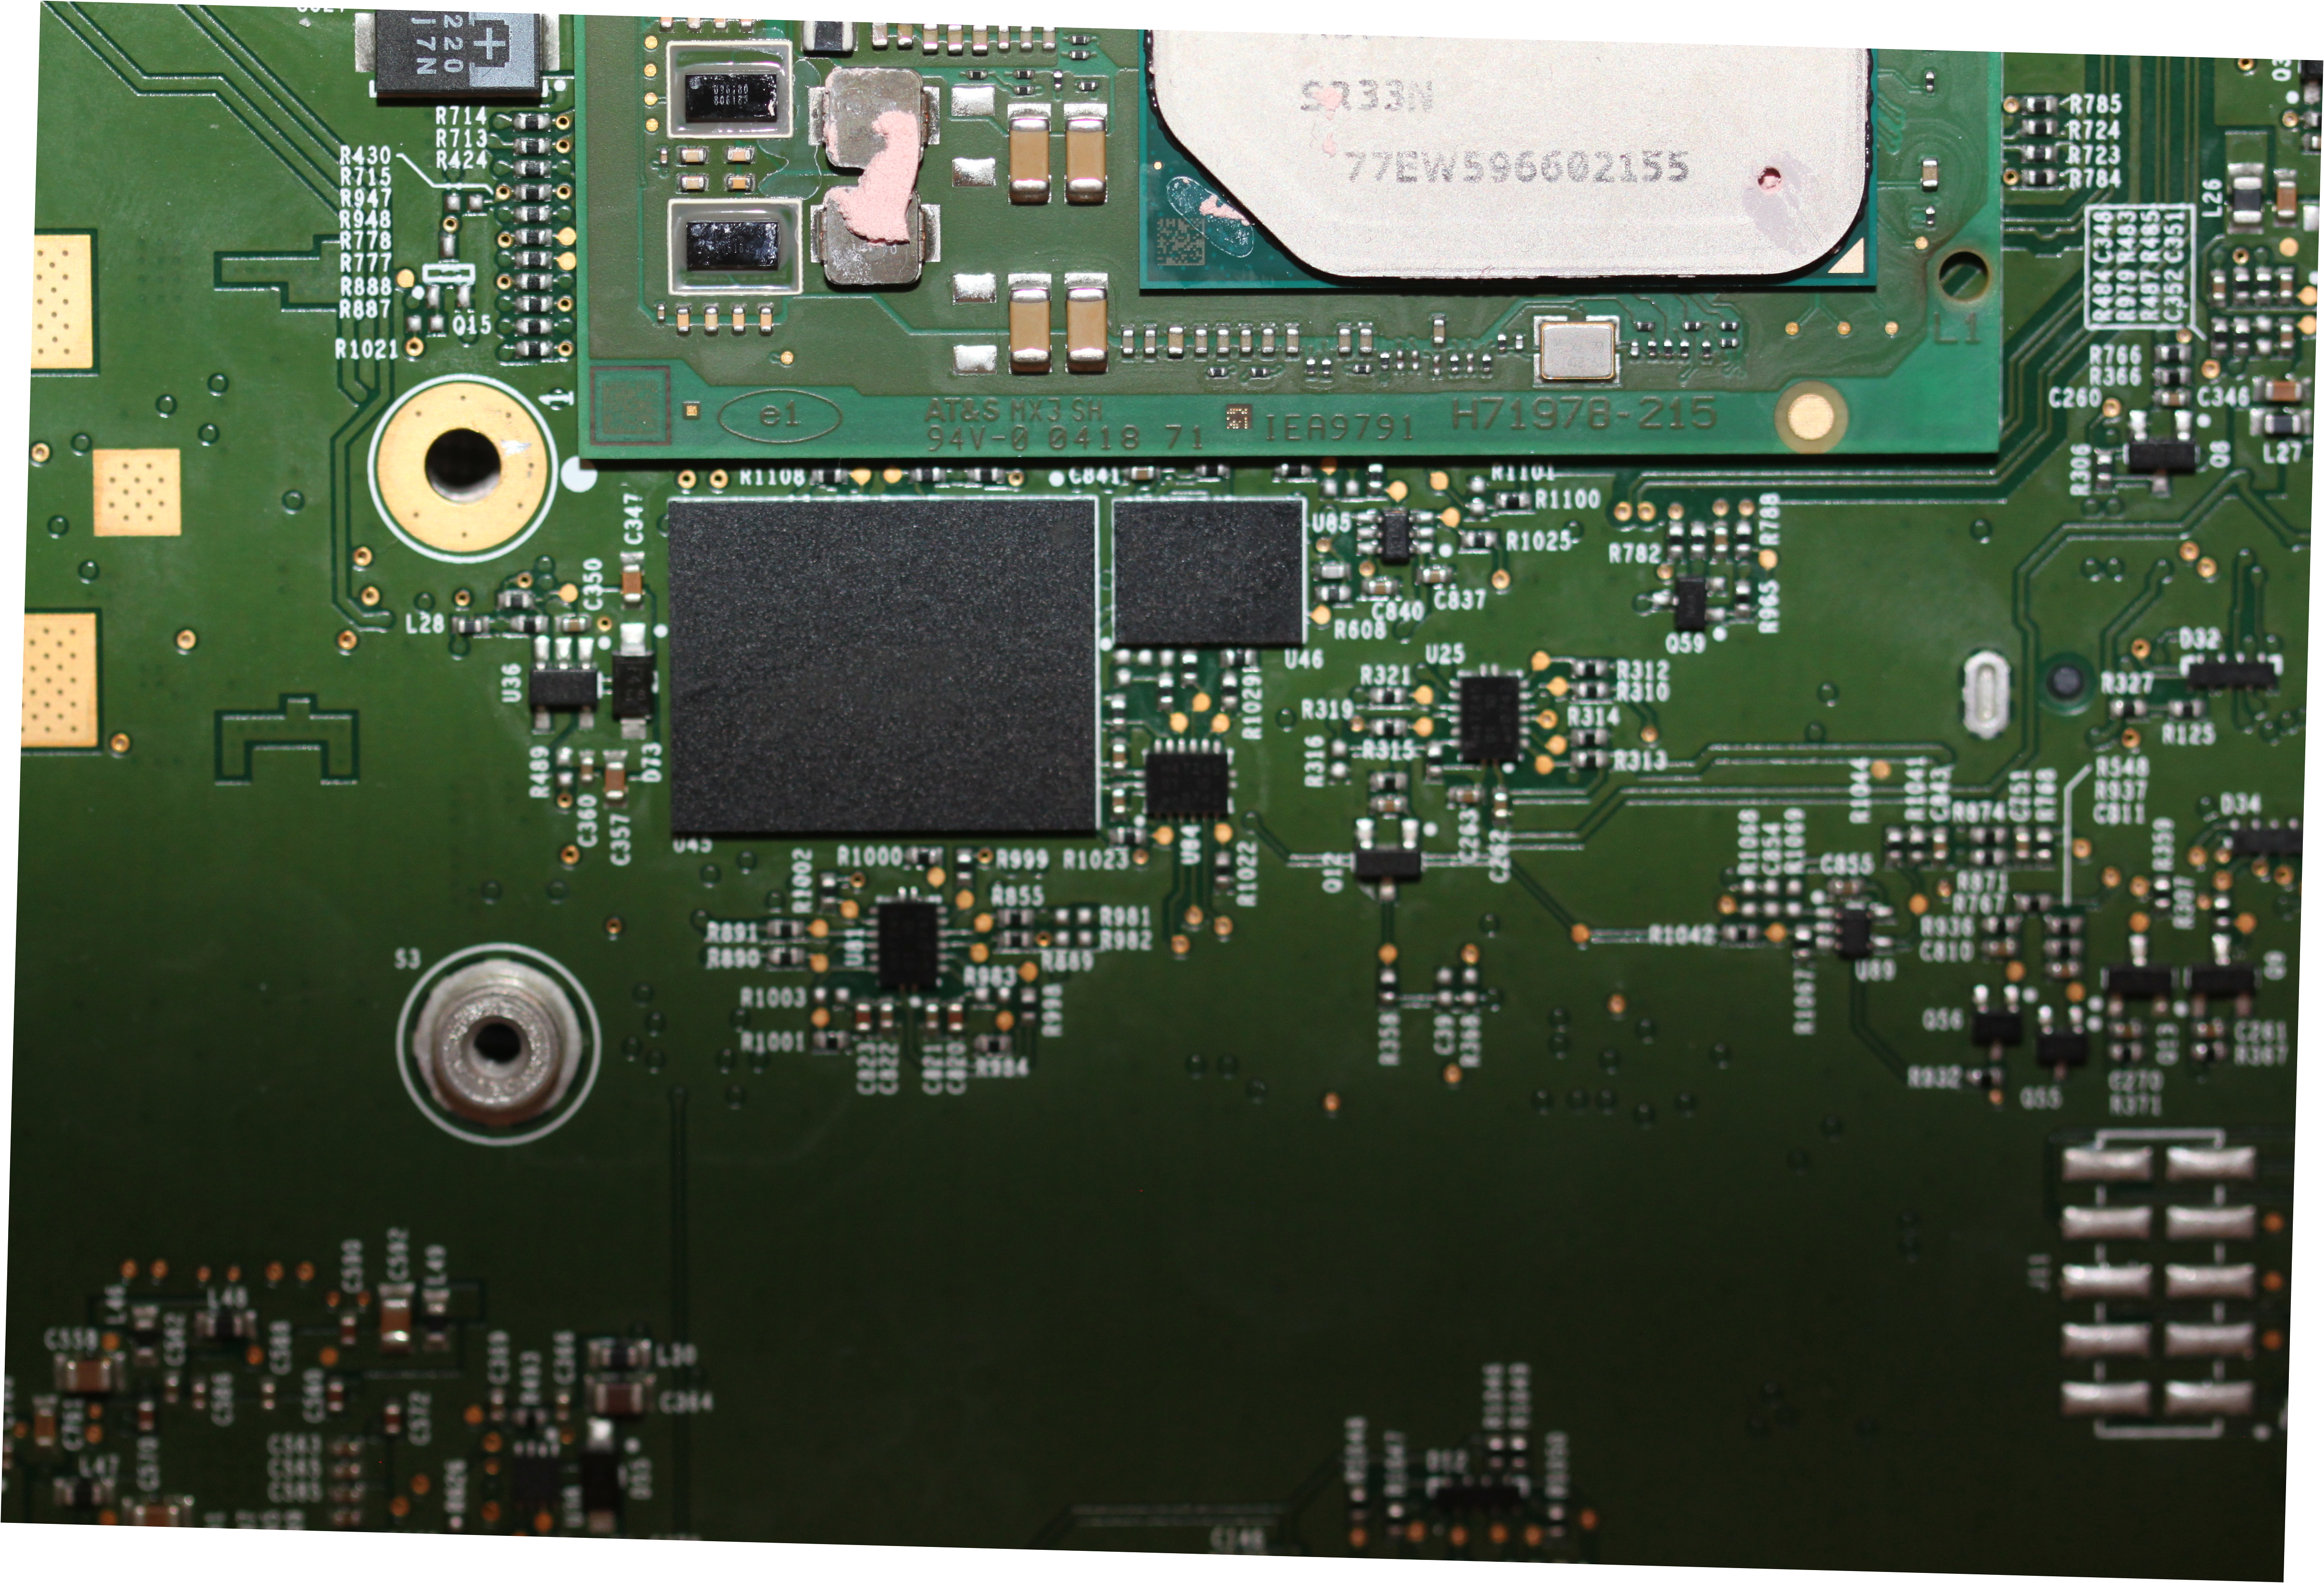
\includegraphics[clip, trim={30cm 25cm 45cm 25cm}, width=1\textwidth]{back.jpg}

	\begin{tikzpicture}[overlay] , show background grid]
		\node[pindot, draw=orange] (D3target) at (-7.80, 7.13) {};
		\node[orange] (D3) at (-6.5, 6.13) {D3};
		\path[draw, ->, orange, thick] (D3) to (D3target);

		\node[pindot, draw=cyan] (D5target) at (-8.08, 7.13) {};
		\node[cyan] (D5) at (-9.5, 6.13) {D5};
		\path[draw, ->, cyan, thick] (D5) to (D5target);

		\node[pindot, draw=yellow] (CMDtarget) at (-6.65, 7.13) {};
		\node[yellow] (CMD) at (-4.5, 6.13) {CMD};
		\path[draw, ->, yellow, thick] (CMD) to (CMDtarget);

		\node[pindot, draw=pink] (VCCtarget) at (-10.48, 5.78) {};
		\node[pink] (VCC) at (-8.5, 5.18) {$V_{CC}$};
		\path[draw, ->, pink, thick] (VCC) to (VCCtarget);
	\end{tikzpicture}
\end{document}

